\documentclass[12pt]{article}

\usepackage[utf8]{inputenc}
\usepackage{latexsym,amsfonts,amssymb,amsthm,amsmath,graphicx,mathtools,subfig,hyperref,float,bm}
\usepackage[parfill]{parskip}
\usepackage[export]{adjustbox}
\usepackage[justification=centering]{caption}
\usepackage{nameref}
\usepackage{cleveref}

\hypersetup{
    colorlinks=true,
    linkcolor=blue,
    filecolor=magenta,      
    urlcolor=cyan,
}

\DeclareMathAlphabet{\mymathbb}{U}{BOONDOX-ds}{m}{n}

\setlength{\parindent}{0in}
\setlength{\oddsidemargin}{0in}
\setlength{\textwidth}{17cm}
\setlength{\textheight}{22cm}
\setlength{\topmargin}{0cm}
\setlength{\headheight}{0pt}
\setlength{\footskip}{30pt}

\DeclareMathOperator*{\argmax}{arg\,max}
\DeclareMathOperator*{\argmin}{arg\,min}
\DeclareMathOperator*{\proj}{proj}
\DeclareMathOperator*{\lmo}{lmo}
\DeclareMathOperator*{\tr}{Tr}


\renewcommand{\thesubsubsection}{\thesubsection.\alph{subsubsection}}

\newcommand{\boldZ}{\mathbf{Z}}
\newcommand{\boldX}{\mathbf{X}}
\newcommand{\boldU}{\mathbf{U}}
\newcommand{\boldV}{\mathbf{V}}
\newcommand{\setX}{\mathcal{X}}
\newcommand{\boldS}{\mathbf{\Sigma}}
\newcommand{\boldu}{\mathbf{u}}
\newcommand{\boldv}{\mathbf{v}}
\newcommand{\boldb}{\mathbf{b}}
\newcommand{\boldA}{\mathbf{A}}

\title{EE-556 Homework 4}
\author{Edoardo Debenedetti}

\begin{document}

\maketitle

\section{Theory: Projection free convex low-rank matrix optimization}

\subsection{Projection onto the nuclear norm ball}
\subsubsection{Projection proof}
\begin{proof}
Let $\boldZ = \boldU\boldS\boldV^T$ be the SVD of $\boldZ \in \mathbb{R}^{p \times m}$, and $\setX = \{ \boldX : \lVert \boldX \rVert_{*} \leq \kappa \}$, we can write the projection of $\boldZ$ onto $\setX$ as:
\begin{equation}
    \proj_{\setX}(\boldZ) = \argmin_{\boldX \in \setX} \lVert \boldX - \boldZ \rVert_{F}
\end{equation}

Let us first look for the projection, onto $\setX$ of $\boldS$:
\begin{equation}
    \proj_{\setX}(\boldS_{\boldZ}) = \argmin_{\boldS_{\boldX} \in \setX} \lVert \boldS_{\boldX} - \boldS_{\boldZ} \rVert_{F}
\end{equation}
However, given that $\boldS$ is diagonal, its nuclear norm $\lVert \boldS \rVert_{*}$ is the sum of its singular values. However, as $\Sigma$ is diagonal, its singular values are given by the diagonal itself, and their sum is the sum of the diagonal elements. Moreover, its diagonal elements are the only non-zero elements, and then, when computing its $\ell1$-norm $\lVert \boldS \rVert_{1}$, we sum only the absolute value of the diagonal. Moreover, as the entries of $\boldS$ are singular values, they are all non-negative and they are equal to their absolute value. Hence, $\lVert \boldS \rVert_{*} = \lVert \boldS \rVert_{1}$, and, when considering $\boldS$, $\setX = \{ \boldX : \lVert \boldX \rVert_{*} \leq \kappa \} = \{ \boldX : \lVert \boldX \rVert_{1} \leq \kappa \}$. Hence,
\begin{equation}
     \proj_{\setX}(\boldS_{\boldZ}) = \argmin_{\boldS_{\boldX} \in \setX} \lVert \boldS_{\boldX} - \boldS_{\boldZ} \rVert_{F} = \boldS_{\boldZ}^{\ell1}
\end{equation}
where $\boldS_{\boldZ}^{\ell1}$ is the projection of $\boldS_{\boldZ}$ onto the $\ell1$-norm ball smaller than $\kappa$. Moreover, we can state that
\begin{equation}
    \min_{\boldS_{\boldX} \in \setX} \lVert \boldS_{\boldX} - \boldS_{\boldZ} \rVert_{F} = \lVert \boldS_{\boldZ}^{\ell1} - \boldS_{\boldZ} \rVert_{F} \label{eq:sigma-proj}    
\end{equation}
Now let us consider, again, $\lVert \boldX - \boldZ \rVert_{F}$. Thanks to Mirsky's inequality we know that $\lVert \boldX - \boldZ \rVert_{F} \geq \lVert \boldS_{\boldX} - \boldS_{\boldZ} \rVert_{F}$, and then, thanks to \Cref{eq:sigma-proj}, we can state that $\lVert \boldX - \boldZ \rVert_{F} \geq \lVert \boldS_{\boldZ}^{\ell1} - \boldS_{\boldZ} \rVert_{F}$, which means that $\lVert \boldS_{\boldZ}^{\ell1} - \boldS_{\boldZ} \rVert_{F}$ is a lower bound for the projection argument.

If we set $\boldX = \boldU \boldS_{\boldZ}^{\ell1} \boldV^T$, we then have
\begin{gather}
    \lVert \boldU \boldS_{\boldZ}^{\ell1} \boldV^T - \boldU \boldS \boldV^T \rVert = \\
    = \lVert \boldU (\boldS_{\boldZ}^{\ell1} \boldV^T - \boldS \boldV^T) \rVert = \\
    = \lVert \boldU (\boldS_{\boldZ}^{\ell1} - \boldS) \boldV^T \rVert = \label{eq:frob-invariance-1} \\
    = \lVert \boldS_{\boldZ}^{\ell1} - \boldS \rVert \label{eq:frob-invariance-2}
\end{gather}

It is worth noting that between \Cref{eq:frob-invariance-1} and \Cref{eq:frob-invariance-2} we exploted the fact that $\boldU$ and $\boldV$ are unitary matrices and hence orthogonal, and that Frobenius norm is invariant of orthogonal matrices.

We can now note that if we set $\boldX$ as we did above, we get a norm which is equal to a lower-bound, and hence is a minimum, which means that
\begin{equation}
    \boldX = \boldU \boldS_{\boldZ}^{\ell1} \boldV^T \in \argmin_{\boldX \in \setX} \lVert \boldX - \boldZ \rVert_{F} = \proj_{\setX}(\boldZ)
\end{equation}
\end{proof}

\subsubsection{Implementation}
We can observe from \Cref{tab:projections} that the average duration with 1M entries matrix is exponentially larger than that with 100k entries. This is coherent with SVD decomposition complexity, which is exponential: $\mathcal{O}(\min(m^2p, mp^2))$.

\begin{table}[ht]
\centering
\caption{Duration of matrix projections onto the nuclear norm ball with $\kappa = 5000$.}
\label{tab:projections}
\begin{tabular}{ccccccc}
Measure & 1 & 2 & 3 & 4 & 5 & Average \\ \hline
100k (s) & 0.7198 & 0.6789 & 0.6661 & 0.677 & 0.6504 & 0.67844 \\ \hline
1M (s) & 37.6 & 35.4 & 35.42 & 35.27 & 35.25 & 35.788
\end{tabular}
\end{table}

\subsection{LMO of nuclear norm}
\subsubsection{LMO proof}
Given that
\begin{equation}
    \lmo_{\setX}(\boldZ) = \argmin_{\boldX \in \setX} \langle \boldX, \boldZ \rangle
\end{equation}
where $\langle \boldX, \boldZ \rangle = \tr(\boldZ^T\boldX)$, we want to show that
\begin{equation}
    -\kappa \boldu \boldv^T \in \lmo_{\setX}(\boldZ)
\end{equation}
As $\kappa \boldu \boldv^T \in \setX$, we just need to show that $\langle \boldX, \boldZ \rangle \geq \langle -\kappa \boldu \boldv^T, \boldZ \rangle$.

First, let us work on $\langle -\kappa \boldu \boldv^T, \boldZ \rangle$:
\begin{gather}
    \langle \kappa \boldu \boldv^T, \boldZ \rangle = \tr(\boldZ^T (-\kappa \boldu \boldv^T)) = \\
    = -\kappa \tr(\boldZ^T \boldu \boldv^T)
\end{gather}
Thanks to variational characterization of singular vectors, $\boldZ^T \boldu = \sigma \boldv$, where $\sigma$ is the singular value corresponding to the singular vectors $\boldu$ and $\boldv$, i.e. the largest singular value. Hence we get
\begin{gather}
    \langle \kappa \boldu \boldv^T, \boldZ \rangle = -\kappa \tr(\sigma \boldv \boldv^T) = \\
    = -\kappa \sigma \tr(\boldv \boldv^T) = -\kappa \sigma
\end{gather}
Where we leveraged the fact that $\boldv$ is a column of the unitary matrix $\boldV$ and then its inner product with itself $\langle \boldv, \boldv \rangle = \tr(\boldv^T\boldv) = \tr(\boldv\boldv^T) = 1$.

\subsubsection{Implementation}
We can see from \Cref{tab:lmo-durations} that the duration with a 1M entries matrix is less than 10 times larger than the one with 100k entries, which is a significantly smaller ratio than that of projection.

\begin{table}[ht]
\centering
\caption{Duration of LMO computation with $\kappa = 5000.$}
\label{tab:lmo-durations}
\begin{tabular}{lllllll}
Measure & 1 & 2 & 3 & 4 & 5 & Average \\ \hline
100k & 0.1124 & 0.4546 & 0.0401 & 0.0539 & 0.0369 & 0.13958 \\ \hline
1M & 0.7298 & 1.227 & 1.14 & 1.001 & 0.2803 & 0.87562
\end{tabular}
\end{table}

\section{Hands-on experiment 1: Crime Scene Investigation with Blind Deconvolution}

\subsection{Frank-Wolfe for Blind Deconvolution}
\subsubsection{Objective function Lipschitz-smoothness}
\begin{proof}
We first compute the gradient of $f(\boldX) = \frac{1}{2} \lVert \boldA(\boldX) - \boldb \rVert_{2}^{2}$, where $\boldA$ is a linear operator and therefore can be treated as a matrix. The gradient is
\begin{equation}
    \nabla f(\boldX) = \nabla \frac{1}{2} \lVert \boldA(\boldX) - \boldb \rVert_{2}^{2} = \boldA^T(\boldA(\boldX) - \boldb)
\end{equation}
Then, in order to prove the Lipschitz smoothness of the gradient, we need to find a bounded $L$ such that
\begin{equation} \label{eq:lipschitz}
    \lVert \nabla f(\boldX_1) - \nabla f(\boldX_2) \rVert_{2} \leq L \lVert \boldX_1 - \boldX_2 \rVert_{2}
\end{equation}
Let us work on the first term:
\begin{gather}
    \lVert \nabla f(\boldX_1) - \nabla f(\boldX_2) \rVert_{2} = \lVert \boldA^T(\boldA(\boldX_1) - \boldb) - \boldA^T(\boldA(\boldX_2) - \boldb) \rVert_{2} = \\
    = \lVert \boldA^T(\boldA(\boldX_1) - \boldb - \boldA(\boldX_2) + \boldb) \rVert_{2} = \\
    = \lVert \boldA^T\boldA(\boldX_1 - \boldX_2) \rVert_{2} \leq
    \lVert \boldA^T\boldA \rVert_{2 \rightarrow 2} \cdot \lVert \boldX_1 - \boldX_2 \rVert_{2}
\end{gather}
Where we used Cauchy-Schwartz inequality. As $\lVert \boldA^T\boldA \rVert_{2 \rightarrow 2}$ is bounded, \Cref{eq:lipschitz} is satisfied.
\end{proof}

\subsection{Implementation}
As can be seen from

\begin{figure}[ht]
    \centering
    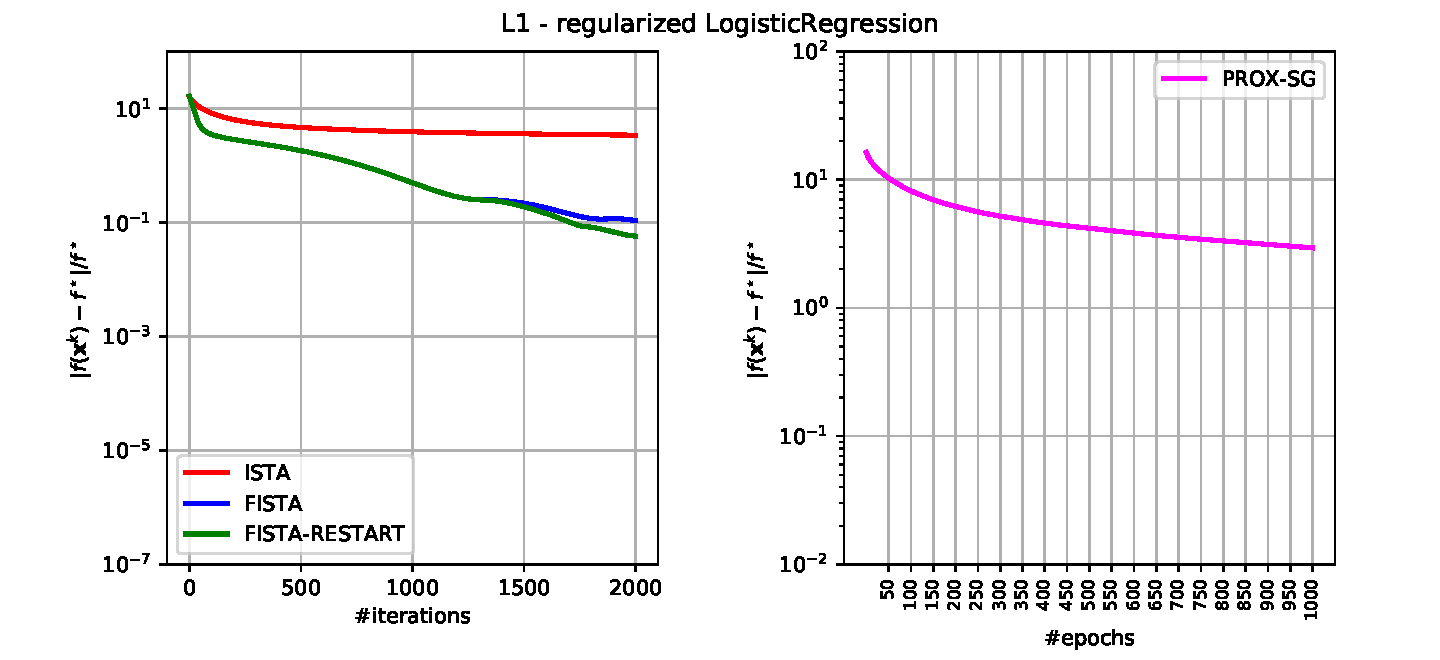
\includegraphics[width=17cm]{hw4/codes/exercise1/results/l1.pdf}
    \caption{Convergence of $\ell$-1 regularized Logistic Regression}
    \label{fig:l1-convergence}
\end{figure}

\section{Hands-on experiment 2: k-means Clustering by Semidefinite Programming}

\subsection{Conditional Gradient Method for Clustering Fashion-MNIST data}
\subsubsection{Domain convexity}
\subsubsection{Penalized objective and gradient}
\subsubsection{\texorpdfstring{$v_{k}$}{Lg} derivation}
\subsubsection{Implementation}

\end{document}